This section is divided into two parts. In \autoref{sec:method-WMF_tool}, we describe the WasteAndMaterialFootprint tool, in \autoref{sec:method-case_study}, we describe the methodology used to calculate the waste and material footprints in the case study.

\subsection{The WasteAndMaterialFootprint tool}
\label{sec:method-WMF_tool}

The WasteAndMaterialFootprint tool is a Python package that allows one to calculate the waste and material footprint of any product or service inside of LCA databases. The tool is built on the \texttt{Brightway2} LCA framework~\citep{mutel2017brightway} and is also compatible with \texttt{ActivityBrowser}~\citep{steubing2020activitybrowser} an open-source graphical user interface for LCA. The WMF tool is installable via the Python Package Index (PyPI)~\citep{mcdowall2023wmfpipy} and is open source under the CC-0 licence. The full source code for the WasteAndMaterialFootprint tool is indexed on Zenodo~\citep{mcdowall2023wmfzenodo} and under further development in the GitHub repository~\citep{mcdowall2024wmfgithub}. The tool is designed to be used with ecoinvent databases~\citep{ecoinvent2016version3}, but could be adapted to other databases as well by changing the search criteria. Currently, it has been tested with all available system models of ecoinvent 3.5--3.10.

The program can be used directly from the command line, or imported as a Python module, in which case, the user can access the individual functions and modules. In the simplest case, the user can run the program with the default settings, which will calculate the waste and material footprint of the ecoinvent database. The user can also customise the program to calculate the waste and material footprint of a custom database, or a prospective database based on future scenarios. The program is designed to be modular so that the user can easily customise the program to their needs.

The following lists outline the constituent modules of the WMF tool, with a brief description of their functions. More extensive details can be found in the user guide and documentation of the program~\citep{mcdowall2023wmfdocs}.

\subsubsection{Functional modules}
\begin{itemize}
    \item \texttt{future\_scenarios}: Creates prospective LCA databases based on future scenarios.
    \item \texttt{explode\_database}: Responsible for expanding a Brightway2 database into detailed exchange lists.
    \item \texttt{search\_waste}: Provides functions for searching and categorising waste generation-related exchange data.
    \item \texttt{search\_material}: Provides functions for searching and categorising material demand-related exchange data.
    \item \texttt{make\_custom\_database}: Facilitates the creation of custom databases based on the waste and material search categories.
    \item \texttt{method\_editor}: Manages the custom LCIA methods for waste and material footprint calculations.
    \item \texttt{exchange\_editor}: Appends `pseudo-biosphere' exchanges to activities to match their waste generation and material demand exchanges in the technosphere.
    \item \texttt{verify\_database}: Performs verification of the manipulated databases.
\end{itemize}

\subsubsection{Configuration modules}
\begin{itemize}
    \item \texttt{custom\_config}: Provides functions for managing the configuration of the WasteAndMaterialFootprint package.
    \item \texttt{user\_settings}: The main configuration file, for defining the project and database settings (user editable).
    \item \texttt{queries\_waste}: Defines search parameters and categories for waste generation exchanges (user editable).
    \item \texttt{queries\_materials}: Defines search parameters and categories for material demand exchanges (user editable).
\end{itemize}

\autoref{fig:WMF_flowchart} shows the flowchart of the WasteAndMaterialFootprint tool. The subsequent subsections describe the computational framework and the modules in more detail.

\begin{figure}[h!]
    \centering
    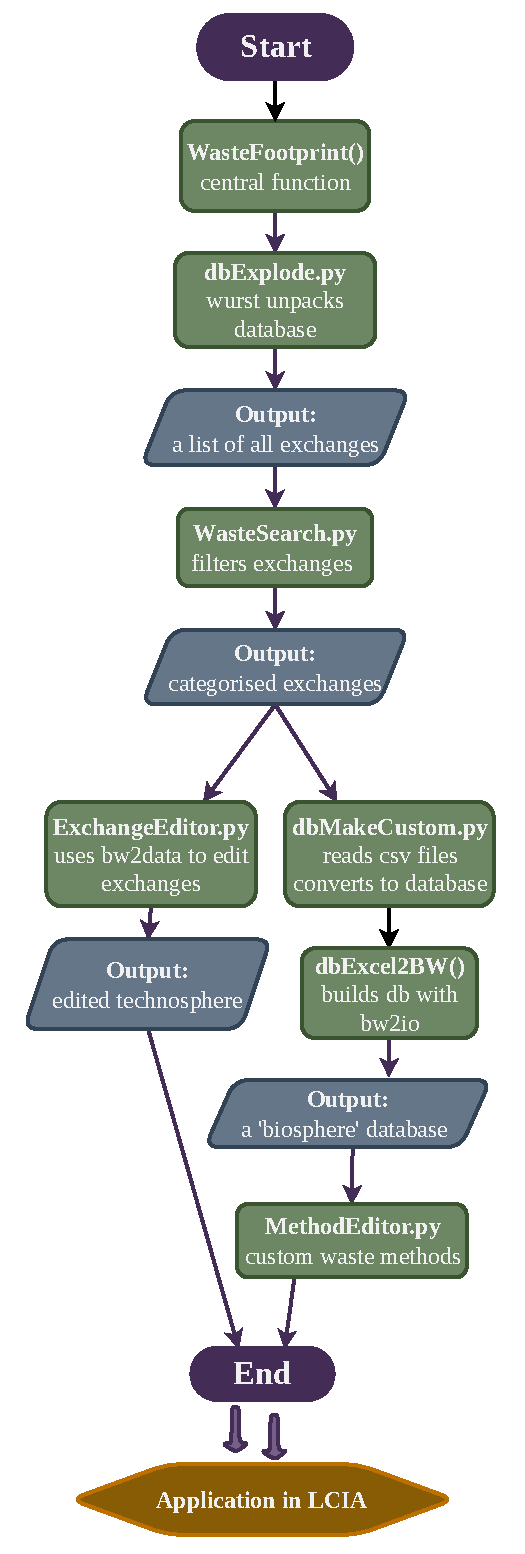
\includegraphics[width=0.7\columnwidth]{figures/WMF_flowchart.pdf}
    \caption{Flowchart of the WasteAndMaterialFootprint tool \cbox{Figure needs to be updated with new names + premise}}\label{fig:WMF_flowchart}
\end{figure}

\subsubsection{Computational framework}
Developed in the Python programming language (version 3), the WMF tool extends the brightway2 LCA framework, utilising the components \texttt{bw2data}, \texttt{bw2calc}, and \texttt{bw2io}~\citep{mutel2017brightway}. Additionally, the \texttt{wurst} package is used to facilitate database searching and data transformation at the exchange level~\citep{mutel2017wurst}. Integration with \texttt{premise} package~\citep{sacchi2022premise} enables the user to easily create and manipulate prospective LCA databases. 


\subsubsection{Generation of prospective LCA databases}
Future waste and material footprints can be projected using the \texttt{future\_scenarios} module, which uses \texttt{premise} to generate prospective scenario databases based on the configuration in \texttt{user\_settings}. These prospective databases can be custom-defined by the user or can be constructed with the future projections of the integrated assessment models such as IMAGE~\citep{stehfest2014image} and REMIND~\citep{remind2020model}, which offer a range of options aligned with the Shared Socioeconomic Pathways (SSPs)~\citep{ssp2020ghg}  that can be paired with a variety of mitigation scenarios.

\subsubsection{Database expansion}
The \texttt{explode\_database} module uses \texttt{wurst} to deconstruct LCA databases into a list of individual exchanges representing all of material and energy flows in the technosphere model. This dataset being converted into a pandas DataFrame and stored as a binary \texttt{.pickle} file for subsequent analysis.

\subsubsection{Waste and material flow identification and categorisation}

The \texttt{search\_waste} and \texttt{search\_material} modules apply user-defined search parameters from \texttt{queries\_waste} and \texttt{queries\_materials} to identify relevant waste and material flows in the list of technosphere exchanges generated by \texttt{explode\_database} and categorises them accordingly. The results of the search functions are stored in \texttt{.csv} files for subsequent use in the WMF tool's workflow.

\subsubsection{Waste exchanges}\label{sec:method-wmf-waste_exchanges}

In the default configuration, there are 10 waste categories which are further divided by their unit of measurement (kilograms and cubic meters) to create a total of 20 waste methods. The waste categories are:
\begin{itemize}[itemsep=0pt]
    \item digestion
    \item composting
    \item open burning
    \item incineration
    \item recycling
    \item landfill
    \item hazardous
    \item non-hazardous
    \item carbon dioxide 
    \item total
\end{itemize}

The logic of screening for waste exchanges is based on a set of boolean search queries (`AND', `OR', and `NOT') that are applied in a list comprehension to the names of every exchange in the LCA database (see `search\_queries.py' for the full list). In this way, the search queries enable classification into categories (such as `hazardous solid' and `incineration liquid') and permit the identification of waste exchanges in addition to those directly connected to waste treatment processes. The search queries are tailored to the specific database and the user can easily modify them to suit their needs. In the default settings, there are a total of 18 waste classifications (9 categories, each separated into liquid and solid waste) For example, the identification of `non-hazardous solid' waste exchanges is based on the following search query; \texttt{AND = [`waste'], NOT = [`hazardous', `radioactive'], UNIT = [`kilogram']} (this can also be inferred and confirmed by comparison with the difference between the results of `total solid' and `hazardous solid').\ \autoref{tab:wf_results} presents a list of waste exchanges identified in the prospective database built from `ecoinvent 3.9.1' according to the IAM model `REMIND' with the RCP `PkBudg500' in the year 2100. Note that the carbon dioxide waste category does not include emissions to the atmosphere. This category is based solely on the accounting of carbon capture and storage (CCS), which is included in many prospective databases as direct sequestration in reservoirs as well as solvent capture.

\begin{table}[ht]
    \centering
    \caption{WasteFootprint search results for the database `ecoinvent cutoff 3.9.1, REMIND, SSP2, PkBudg500, 2100'.}\label{tab:wf_results}
    \begin{tabular}{llr}
        \toprule
        \textbf{Waste exchanges} & \textbf{Unit} & \textbf{Exchange count} \\
        \midrule
        digestion & kilogram & 4 \\
        composting & kilogram & 26 \\
        open burning & kilogram & 535 \\
        incineration & kilogram & 2171 \\
        recycling & kilogram & 137 \\
        landfill & kilogram & 1530 \\
        hazardous & kilogram & 1928 \\
        carbon dioxide & kilogram & 119 \\
        total & kilogram & 29524 \\
        digestion & cubic meter & 16 \\
        composting & cubic meter & 0 \\
        open burning & cubic meter & 0 \\
        incineration & cubic meter & 2 \\
        recycling & cubic meter & 0 \\
        landfill & cubic meter & 2 \\
        hazardous & cubic meter & 437 \\
        carbon dioxide & cubic meter & 0 \\
        total & cubic meter & 4360 \\
        \bottomrule
\end{tabular}
\end{table}

\subsubsection{Material exchanges}\label{sec:method-wmf-material_exchanges}
In addition to the waste categories, the \texttt{queries\_materials} module defines the material demand categories, which are based on the EU Critical Raw Materials (CRM) list for 2023~\citep{eu2023crmstudy}. The CRM list is a list of 30 materials that are considered critical to the EU economy and are at risk of supply disruption. Further materials of interest were added to the search list, including helium, electricity, petroleum, sand, water, and natural gas. The identity of the materials considered and their categorical groupings are easily customisable by the user. A full list of 59 materials included in the default configuration is provided in the supplementary material.

The logic for the identification of material exchanges with the WMF tool differs from that used to identify waste exchanges in that the search queries are based on the names of the so-called relevant `market activities' for the material of interest. That is, for material $x$, all exchanges with the name `market for material $x$' are identified and subsequently apportioned a (`pseudo-biosphere') material demand exchange of the same sign and magnitude as the original exchange. A useful feature of the WMF tool is that, in cases where there are several markets for one material or material group, the program can easily aggregate these exchanges. For example, exchanges with markets for the rare-earth-elements (REEs) `market for cerium', `market for dysprosium', `market for erbium', etc.\ can be aggregated into a single indicator category for REEs. Similarly, the total demand for all critical raw materials (CRMs) can be easily calculated in the same manner. 

As discussed in the introduction~\ref{sec:introduction} there are some existing material demand methods in the standard LCIA method sets, including the `crustal scarcity indicator' (which provides only an aggregated, abstracted endpoint)~\citep{arvidsson2020csi} and the (deprecated) EDIP 2003 material use indicators (which provide endpoints in fundamental units)~\citep{hauschild2003edip}. In these methods, the material demand is calculated based on the total mass that is extracted from the environment, thus, their focus is essentially solely on the mining-related exchanges that bring these materials from the biosphere into the technosphere. In the WMF tool, however, the accounting for material demand is based on exchanges solely within the technosphere. This offers a different perspective, allowing for the estimation of overall supply-chain material demands that consider the entire life cycle of an activity, including non-direct impacts on the market such as co-production of other materials. Consider a demand for an activity containing a metal, for example; while the existing material use methods allow one to calculate the total mass of that metal that is extracted from the environment, the WMF tool can provide insight into the broader supply-chain impacts of the demand for this metal. If the production other materials are attributed to the production of this metal, these would appear as negative material demands in the WMF results---supply chain pressure for one material can result in lessening of supply chain pressure for another. In the results of the Li-ion battery case study in \autoref{sec:results-case_study}, we will see that this is indeed the case for the demand for nickel, which, because of such effects, is counter-intuitively negative despite the presence of nickel in the final products.


\subsubsection{Creation of custom `pseudo-biosphere' databases}
Custom `pseudo-biosphere' databases are created by \texttt{make\_custom\_database} module. This module collates the waste and material categories that were present in the databases, producing an \texttt{.xlsx} file that is imported back into the Brightway2 project as a biosphere-database named `WasteAndMaterialFootprint'. 

\subsubsection{LCIA method management}
The \texttt{method\_editor} module manages the addition, deletion, and verification of the custom LCIA methods used in the WMF tool. This module uses the custom `pseudo-biosphere' databases created by \texttt{make\_custom\_database} to create these waste and material footprint LCIA methods that have the same unit as the respective technosphere exchange. The methods are stored in the Brightway2 project and can be used for calculating the waste and material footprints of activities in the LCA database in the same way as with other LCIA methods. Since `waste is not a service'~\citep{guinee2021wasteisnotaservice}, a characterisation factor of -1 is applied to the waste footprint methods (with the exception of CCS exchanges), changing the perspective from waste consumed by treatment to waste generated by the activity.

\subsection{Exchange editing}
The \texttt{exchange\_editor} module loads the \texttt{.csv} files created by the search functions and appends `pseudo-biosphere' exchanges to the matching activities in the LCA database. This is the most computationally intensive part of the WMF tool, as (depending on the search configuration) there are generally more than 100,000 exchanges to be appended to the database. 

\subsubsection{Database Verification}
The \texttt{verify\_database} module calculates LCA scores for randomly selected activities using Waste Footprint and Material Demand Footprint methods to confirm that the WMF tool has processed the database correctly.

\subsection{Case Study Methodology}\label{sec:method-case_study}

\subsubsection{Activities}
This case study investigated five types of Li-ion batteries, each represented by specific market activities:
\begin{itemize}[itemsep=0pt]
    \item Li-ion, NMC111, rechargeable, prismatic
    \item Li-ion, LiMn2O4, rechargeable, prismatic
    \item Li-ion, NCA, rechargeable, prismatic
    \item Li-ion, NMC811, rechargeable, prismatic
    \item Li-ion, LFP, rechargeable, prismatic
\end{itemize}

\subsubsection{Methods}
In addition to the Waste Footprint and Material Demand footprint methods created by the WMF tool, the following standard LCIA methods were applied for comparison:
\begin{itemize}[itemsep=0pt]
    \item ReCiPe 2016 v1.03, midpoint (I)
    \item EF v3.0 no LT
    \item EDIP 2003 no LT
    \item Crustal Scarcity
\end{itemize}

\subsubsection{Databases}
The primary source of life cycle inventory data for this case study was ecoinvent 3.9.1 cutoff. Additionally, the WMF tool was used to create prospective database sets using the \mbox{REMIND} model with the following Representative Concentration Pathways (RCPs):
\begin{itemize}
    \item \textbf{SSP2 -base:}\\ representing ca. 3.5°C increase in global temperatures to 2100
    \item \textbf{SSP2-PkBudg500:}\\ meeting Paris climate goals, ca. 1.3°C increase to 2100
\end{itemize}

For each pathway, databases were created with texttt{premise}~\citep{sacchi2022premise} and processed with the WMF tool over the time series: 2020, 2040, 2060, 2080, 2100.

\subsubsection{Calculations}
For each combination of activity, method, and database, a single score `LCIA' was calculated along with details of the top contributing processes. Additionally, for the Waste and Material Footprint methods, a contribution analysis was performed. This involved utilizing the \texttt{bwa.compare\_activities\_by\_grouped\_leaves} function from the \texttt{brightway2\_analyzer} package~\cite{mutel2016brightway2analyzer}, an additional component of the Brightway2 LCA framework. This function performs graph traversal on the impact matrix of the LCA object to a specified cutoff and groups the resulting leaves by their CPC codes. This provides insight into the products and sectors in the supply chain of the activity that carry the most responsibility for the final footprint.


